\documentclass[aspectratio=169]{beamer}

\usetheme{HGF}

\usepackage{amsmath}
\usepackage{caption}
\usepackage[utf8x]{inputenc}
\usepackage{graphicx}
\usepackage{pgfplots}
\usepackage{textcomp}
\usepackage{tikz}
\usepackage{xcolor}
\usepackage{xmpmulti}
\usepackage{xpatch}

\xpatchcmd{\itemize}
{\def\makelabel}
{\ifnum\@itemdepth=1\relax
    \setlength\itemsep{2ex}% separation for first level
    \else
    \ifnum\@itemdepth=2\relax
    \setlength\itemsep{1ex}% separation for second level
    \else
    \ifnum\@itemdepth=3\relax
    \setlength\itemsep{0.5ex}% separation for third level
    \fi\fi\fi\def\makelabel
}
{}
{}

\pgfplotsset{compat=newest}

\graphicspath{{./images/}}
\makeatletter
\def\input@path{{./}{./images}}
\makeatother

\newcommand\imageright[1]{ %
    \caption*{\scalebox{.5}{\textcolor{lightgray}{\textcopyright~#1}}} %
}

\DeclareMathOperator*{\argmin}{arg\,min}

\title{Machine Learning with Neural Networks}
\subtitle{GridKa School 2018}
\author{Markus Götz}
\date{2018-08-29}
\institute{KIT}

\begin{document}
    
\section{Introduction}
\label{sec:introduction}

\maketitle

%%%%%%%%%%%%%%%%%%%%%%%%%%%%%%%%%%%%%%%%%%%%%%%%%%%%%%%%%%%%%%%%%%%%%%%%%%%
\begin{frame}
\frametitle{Outline}
    \tableofcontents[hideallsubsections]
\end{frame}

\section{Machine Learning Fundamentals}
\label{sec:machine-learning}

\subsection{Terminology}
\label{subsec:terminology}

\begin{frame}
\frametitle{Terminology}
\begin{columns}
    \begin{column}{0.48\textwidth}
        \begin{itemize}
            \item \textbf{Samples} or instances,\\ 
            individual observations in your data,\\
            e.g. an image, a specimen
            \item \textbf{Features} or attributes,\\ 
            single characteristic of a sample,\\
             e.g. a pixel, measured weight
            \item \textbf{Channels} or time,\\
            depth information,\\
            color channels, change over time
        \end{itemize}
    \end{column}
    \begin{column}{0.48\textwidth}
        \begin{figure}
            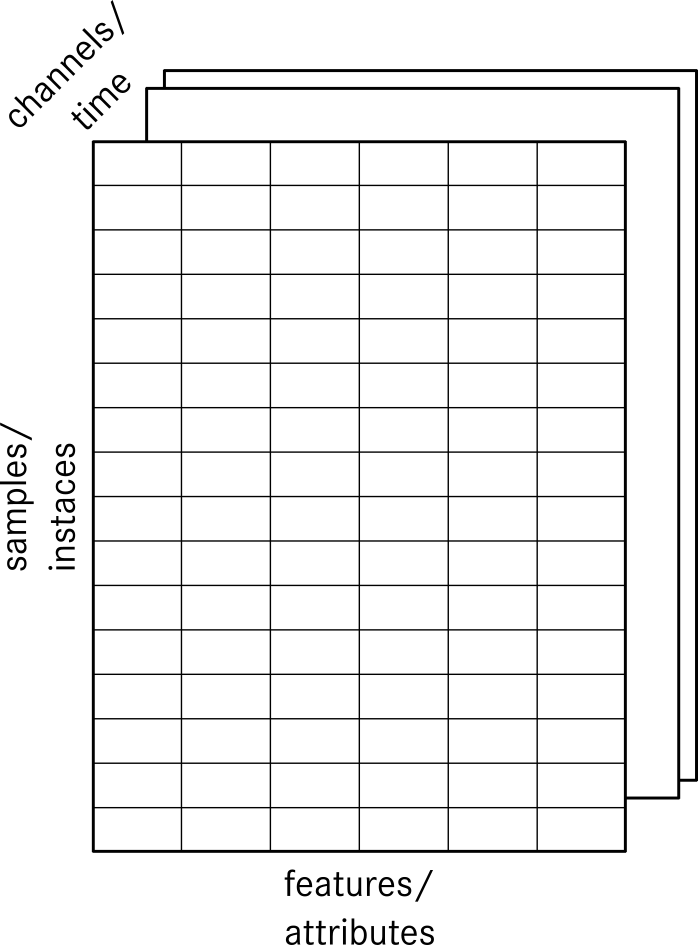
\includegraphics{terminology.png}
        \end{figure}
    \end{column}
\end{columns}
\end{frame}

\begin{frame}
    \frametitle{Terminology}
    \begin{figure}
        \centering
        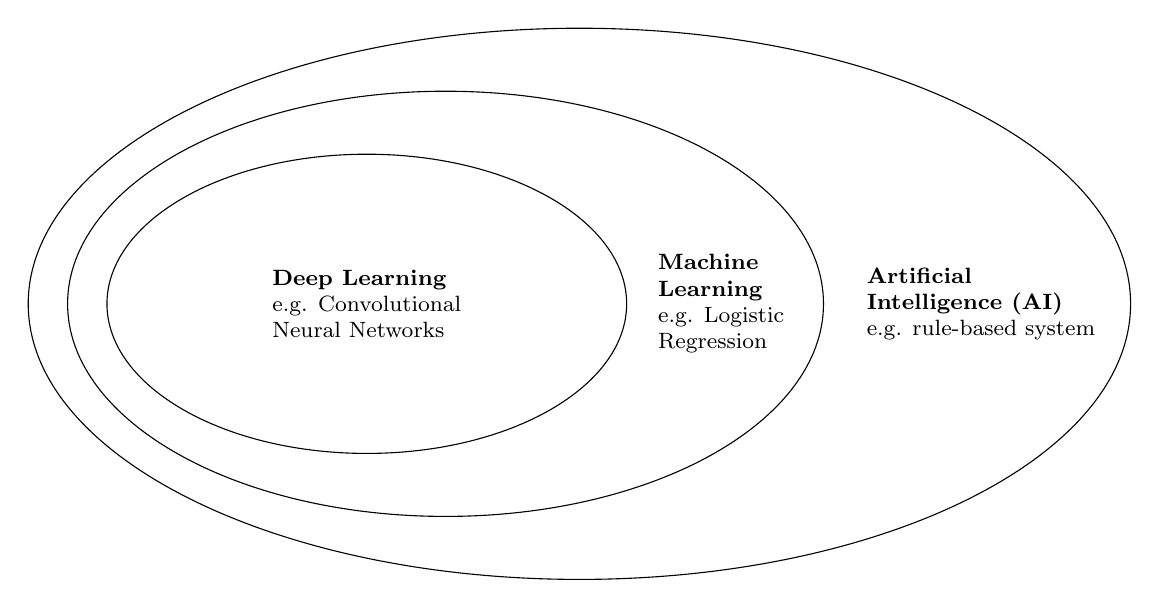
\begin{tikzpicture}[fill=white, font=\footnotesize]
            \draw (0, 0) ellipse (7.0 and 3.5);
            \node[align=left] at (5.1, 0.0) {\textbf{Artificial}\\ \textbf{Intelligence (AI)}\\e.g. rule-based system};
            
            \draw (-1.7, 0) ellipse (4.8 and 2.7) (1.8, 0.0) node[align=left] {\textbf{Machine}\\ \textbf{Learning}\\ e.g. Logistic\\ Regression};
            
            \draw (-2.7, 0) ellipse (3.3 and 1.9) (-2.7, 0.0) node[align=left] {\textbf{Deep Learning}\\ e.g. Convolutional\\ Neural Networks};
        \end{tikzpicture}
    \end{figure}
\end{frame}

\begin{frame}
\frametitle{Terminology}
    \begin{itemize}
        \item \textbf{Supervised learning:} Learn by ``mimicking supervisor'', i.e. pattern annotations\\ 
        examples: image classification, stock forecasting
        \item \textbf{Unsupervised learning:} Determine patterns purely based on data\\ examples: customer cluster analysis, distribution estimation
        \item \textbf{Reinforcement learning:} Pavlov-style learning with punishment and reward in dynamic environments\\
        examples: game AIs, e.g. AlphaGo or Dota OpenAI
    \end{itemize}

    \medskip
\end{frame}

\begin{frame}
\frametitle{Notation Disclaimer}
\begin{itemize}
    \item \textbf{Small letters:} vectors or matrices, e.g. $x$ or $y$
    \item \textbf{Hats:} predictions or estimates, e.g. $\hat{y}$
    \item \textbf{Indices:} elements of vectors and matrices, e.g. $x_{i}$
\end{itemize}

\medskip
\end{frame}

\begin{frame}
\frametitle{Linear Regression}
    \begin{columns}
        \begin{column}{0.43\textwidth}
            \begin{figure}
                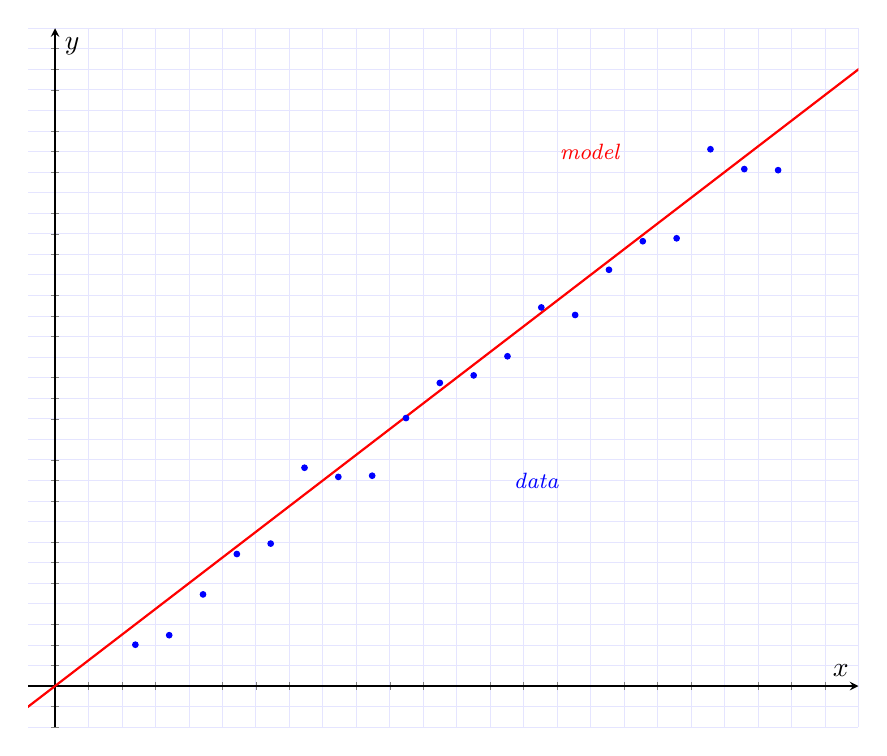
\begin{tikzpicture}
                    \begin{axis}[
                        width=\linewidth, 
                        grid=both,
                        grid style={line width=.3pt, draw=blue!10},
                        major grid style={line width=.3pt, draw=blue!10},
                        minor tick num=3,
                        xlabel={$x$},
                        ylabel={$y$}, 
                        ticks=none,
                        axis x line=center,
                        axis y line=center,
                        xmin=-0.1,
                        xmax=3.0,
                        ymin=-0.1,
                        ymax=1.6
                    ]
                    % domain=0.25:2.75
                    \addplot [red, thick, mark=none] {0.5*x};
                    \node at (axis cs:2.0,1.3) [red] {\footnotesize\emph{model}};
                    \addplot [blue, only marks, mark size=1pt] coordinates {
                        (0.3, 0.10054215032765762)
                        (0.4263157894736842, 0.12363160260273953)
                        (0.5526315789473685, 0.2228985962683488)
                        (0.6789473684210527, 0.32110283680834006)
                        (0.8052631578947369, 0.3464254484709207)
                        (0.9315789473684213, 0.530973472751518)
                        (1.0578947368421054, 0.508700039361571)
                        (1.1842105263157896, 0.5115642913251457)
                        (1.310526315789474, 0.6517708510332498)
                        (1.4368421052631581, 0.7372626388813315)
                        (1.5631578947368425, 0.7555802030144961)
                        (1.6894736842105267, 0.8020873099226213)
                        (1.8157894736842108, 0.920859494738636)
                        (1.9421052631578952, 0.9025123937365214)
                        (2.0684210526315794, 1.0124087289206862)
                        (2.1947368421052635, 1.081906810760111)
                        (2.3210526315789477, 1.089021024213448)
                        (2.447368421052632, 1.3056222105270976)
                        (2.573684210526316, 1.2573605236570795)
                        (2.7, 1.2546989788028189)
                    };
                    \node at (axis cs:1.8,0.5) [blue] {\footnotesize\emph{data}};
                    \end{axis} 
                \end{tikzpicture}
            \end{figure}
        \end{column}
        \begin{column}{0.53\textwidth}
            \begin{itemize}
                \item<1-> \textbf{Data set} $\{samples, labels\}=\{x, y\}$
                \item<2-> \textbf{Model} definition $\hat{y}=wx+b$\\ with $w$ and $b$ trainable parameters
                \item<3-> \textbf{Loss function} or cost/objective\\
                $J(w,b)=MSE(w,b)=\frac{1}{N}\sum_{i=1}^{N}(y_i-\hat{y_i})^2$
                \item<4-> \textbf{Train} the model, e.g. optimization\\
                $\hat{w}, \hat{b}=\argmin J(w, b)$ \\
                
            \end{itemize}
        \end{column}
    \end{columns}

    \bigskip
    \begin{itemize}
        \item<5>
            \begin{center}
                \textbf{Basic recipe for most machine learning algorithms}
            \end{center}
    \end{itemize}
\end{frame}

\subsection{Frameworks}
\label{subsec:frameworks}

\subsection{Exercise: MNIST Dataset}
\label{subsec:fnn-exercise}

\begin{frame}
    \frametitle{Exercise 1: Warm-up}
    \begin{figure}
        \centering
        \begin{tikzpicture}[]
            \node [inner sep=0pt,above right] { %
                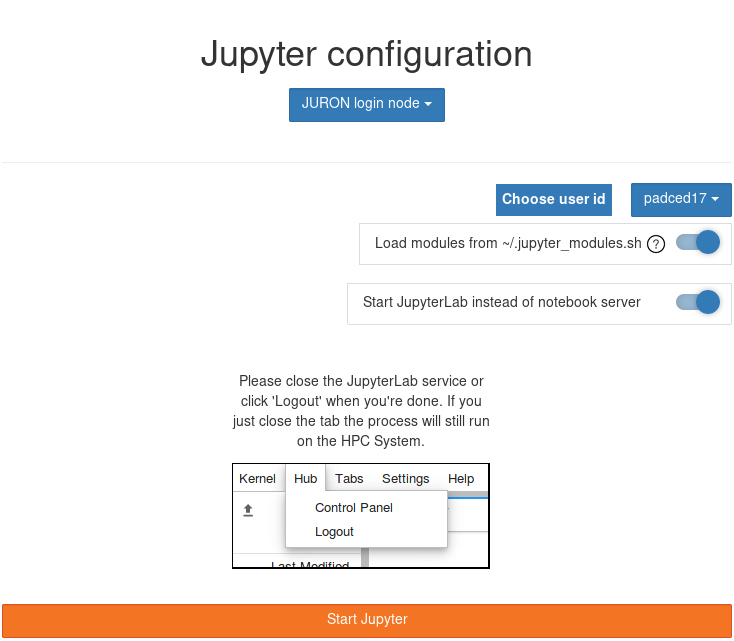
\includegraphics[width=0.5\linewidth]{jupyter.png} %
            };
            % show origin
            \draw [line width=0.6mm, red] (7.05, 4.05) ellipse (0.5 and 0.25);
        \end{tikzpicture}
    \end{figure}
\end{frame}

\subsection{Logistic Regression}
\label{subsec:logistic-regression}

\subsection{Exercise: Logistic Regression}
\label{subsec:exercise-logistic-regression}

\begin{frame}
    \frametitle{Exercise: Logistic Regression}
    \begin{figure}
        \centering
    \end{figure}
\end{frame}

\section{Neural Networks}
\label{sec:neural-networks}

\subsection{Backpropagation}
\label{subsec:Backpropagation}

\subsection{Generalization}
\label{subsec:generalization}

\subsection{Exercise: MNIST FNN}
\label{subsec:exercise-fnn}

\begin{frame}
    \frametitle{Exercise: FNN MNIST Image Classification}
    
    \begin{figure}
        \centering
        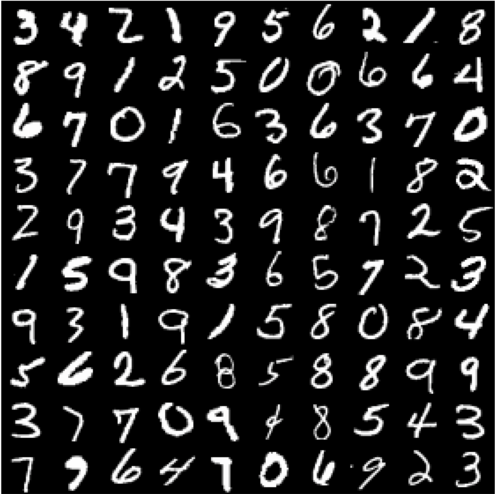
\includegraphics[width=0.4\linewidth]{mnist.png}
    \end{figure}
\end{frame}

\section{Convolutional Neural Networks}
\label{sec:convolutional-neural-networks}

\subsection{Discrete Convolution}
\label{subsec:discrete-convolution}

\begin{frame}
    \frametitle{Discrete Convolution}
    \begin{figure}
        \centering
        \multiinclude[<+->][format=png, graphics={width=0.8\linewidth}]{convolution}
        \imageright{Machine Learning Guru}
    \end{figure}
\end{frame}

\subsection{Network Architectures}
\label{subsec:network-architectures}

\subsection{Exercise: MNIST CNN}
\label{subsec:cnn-exercise}

\begin{frame}
\frametitle{Exercise: FNN MNIST Image Classification}

\begin{figure}
    \centering
    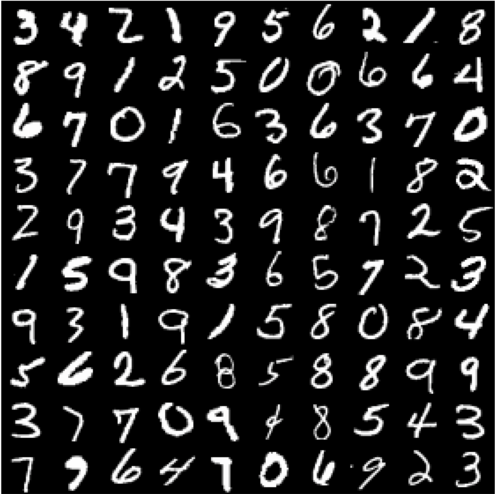
\includegraphics[width=0.4\linewidth]{mnist.png}
\end{figure}
\end{frame}

\section{Regression}
\label{sec:regression}

\subsection{Exercise: Abalone}
\label{subsec:regression-exercise}

\begin{frame}
    \frametitle{Exercise: Abalone Age Regression Analysis}
    \begin{figure}
        \centering
        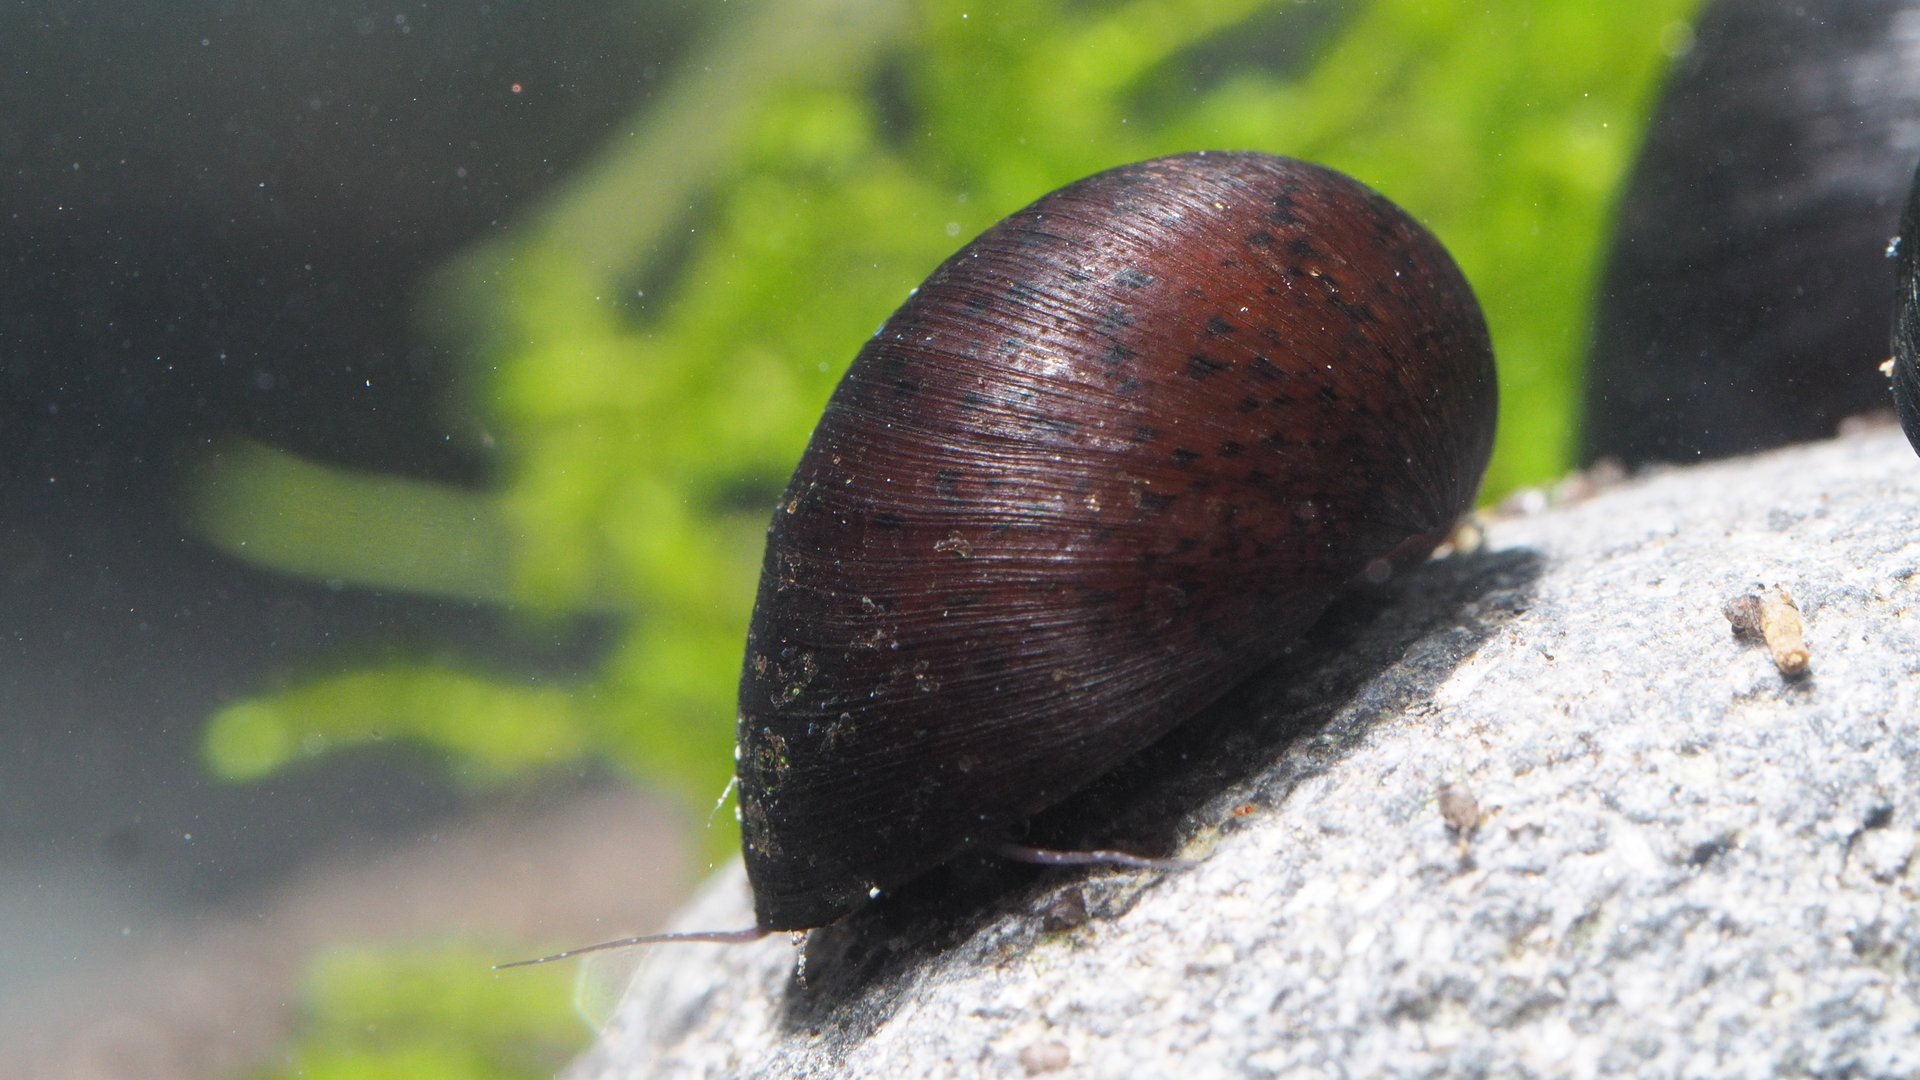
\includegraphics[width=0.7\linewidth]{abalone.jpg}
        \imageright{Garnelaxia}
    \end{figure}
\end{frame}

\section{Summary}
\label{sec:summary}


\begin{frame}
\frametitle{Summary}
\end{frame}

\begin{frame}
\frametitle{Open Topics}
\end{frame}

\begin{frame}
\frametitle{Acknowledgment}

\begin{columns}
    \begin{column}{0.48\textwidth}
        \begin{itemize}
            \item \textbf{Eileen Kühn}
            \begin{itemize}
                \item GridKa School organization
                \item Administrative paperwork
            \end{itemize}
            \item \textbf{Oskar Taubert}
            \begin{itemize}
                \item Assignment preparation
                \item Exercise supervision
            \end{itemize}
            \item \textbf{Andreas Herten}
            \begin{itemize}
                \item Access to JURON
                \item Technical support
            \end{itemize}
        \end{itemize}
    \end{column}

    \begin{column}{0.48\textwidth}
        \begin{figure}
            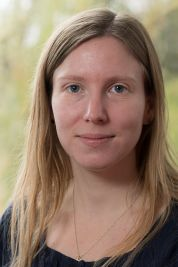
\includegraphics[width=0.25\linewidth]{eileen.jpg}\quad 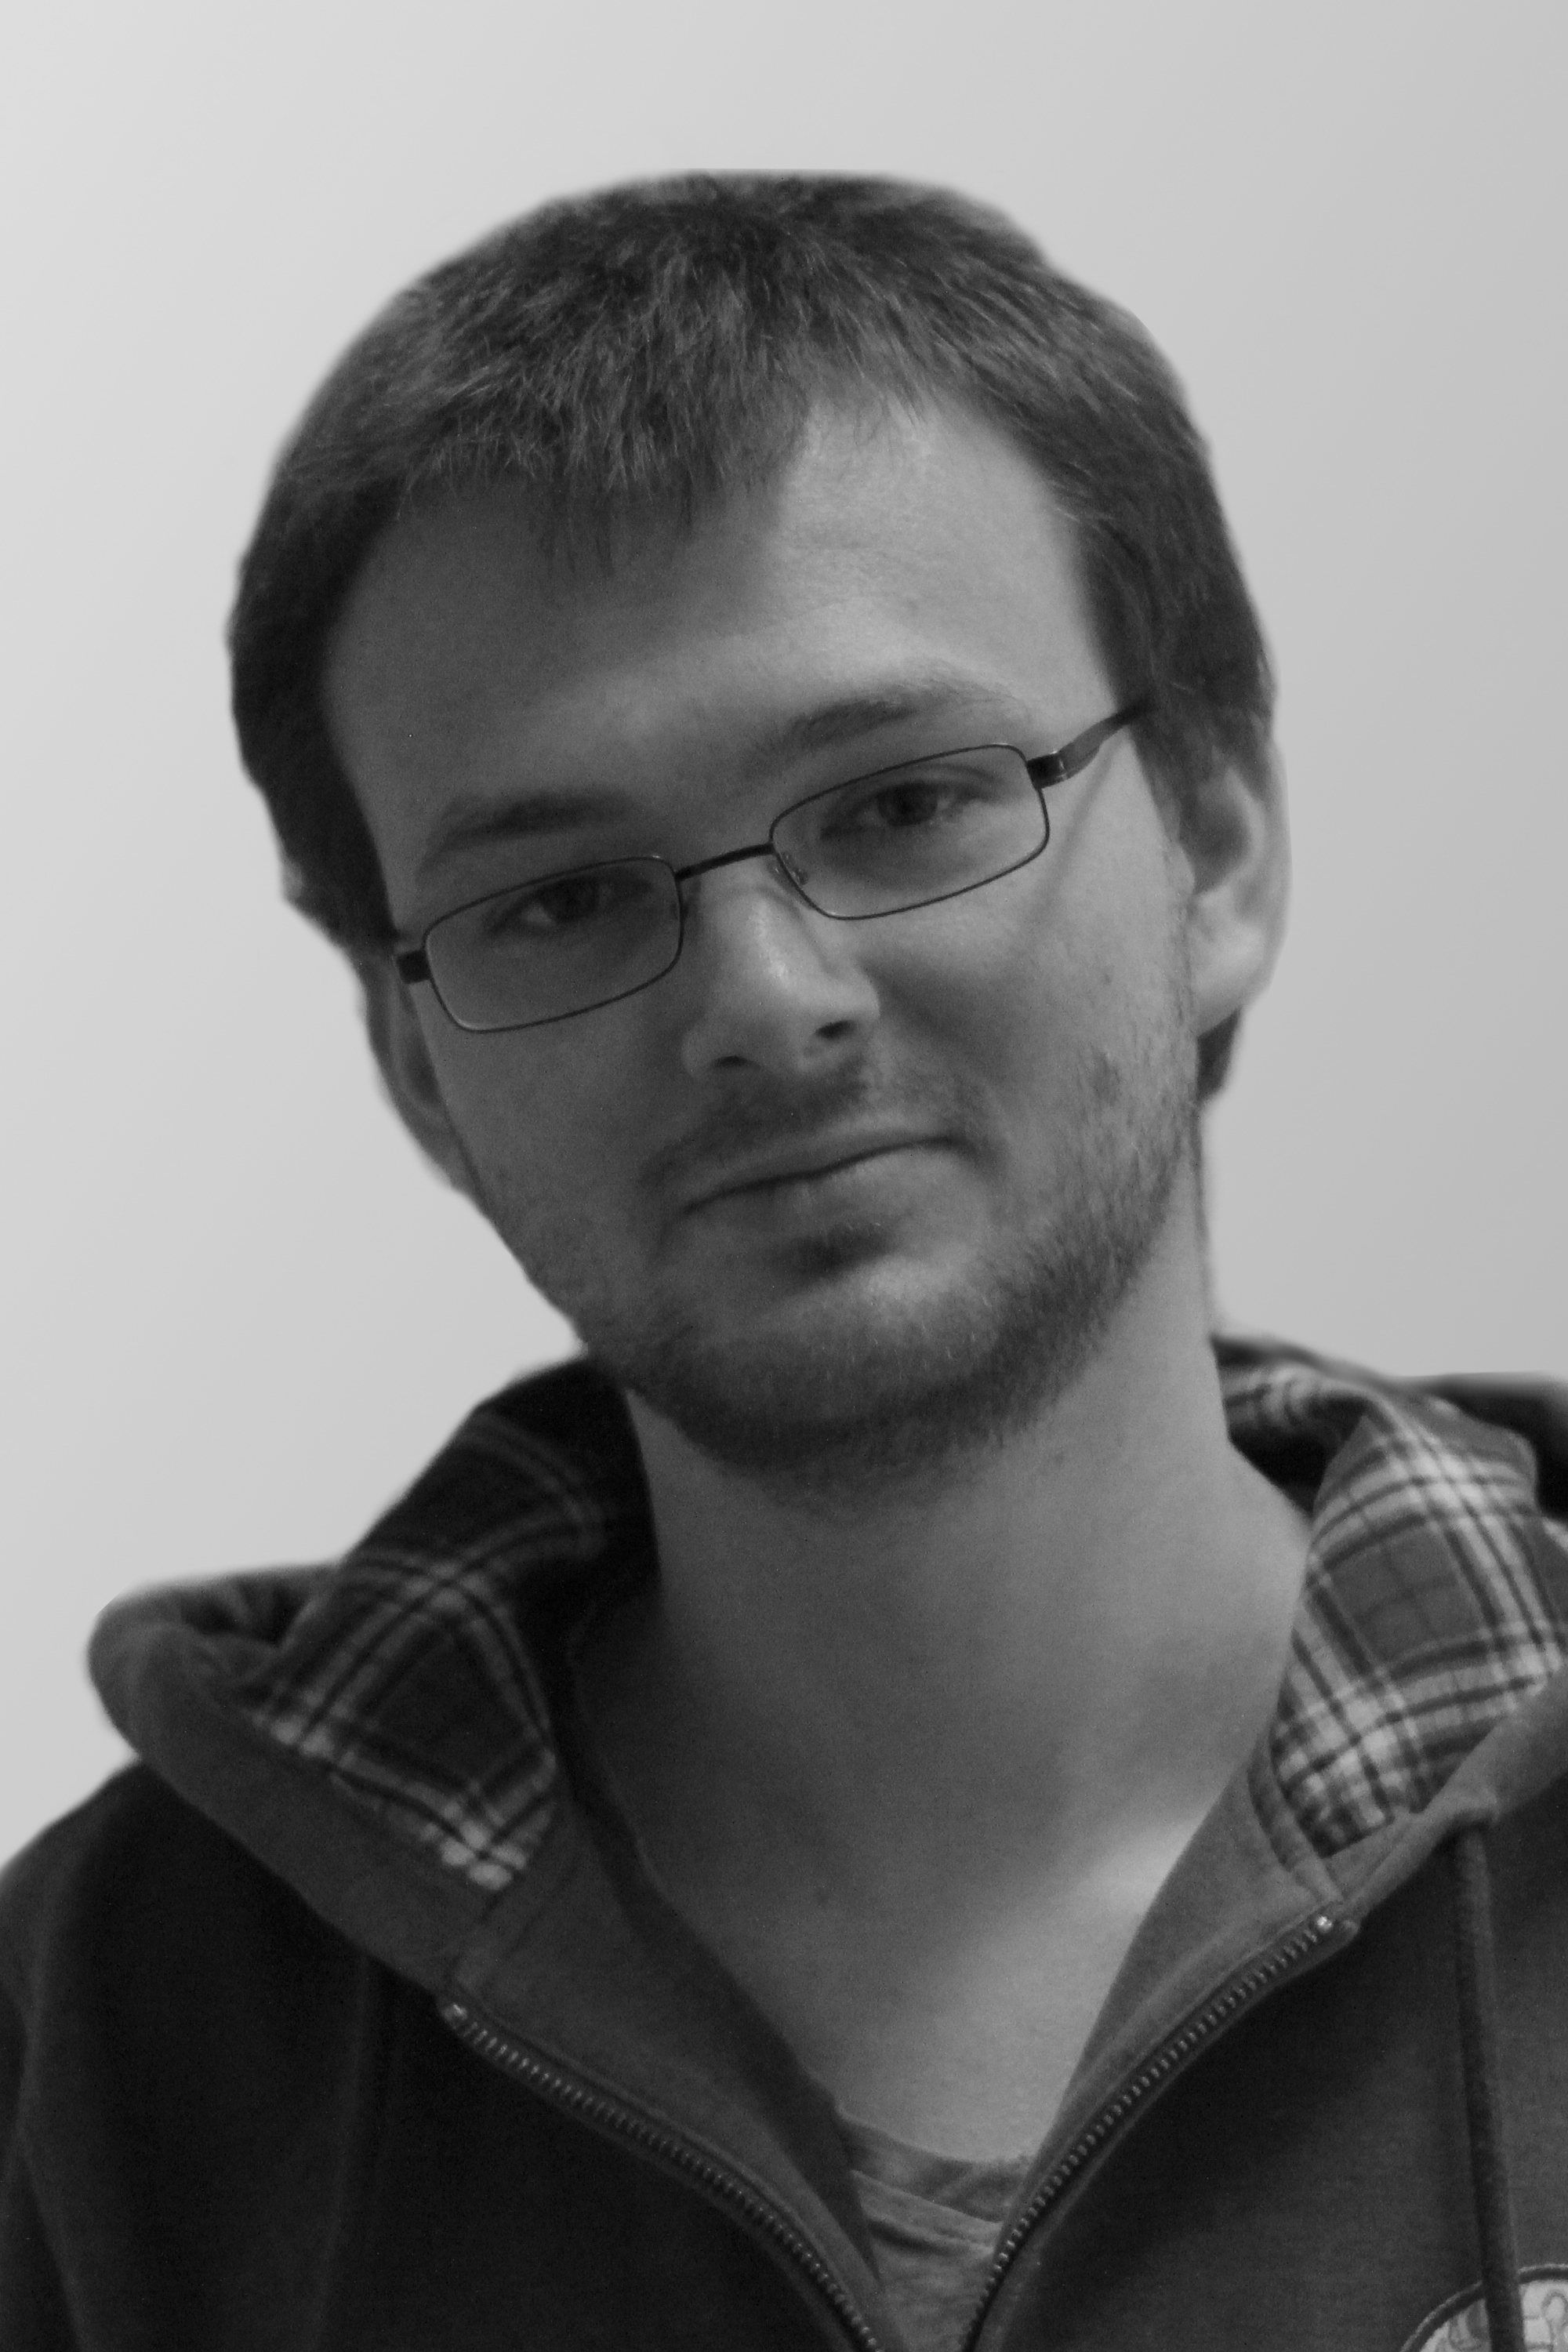
\includegraphics[width=0.25\linewidth]{oskar.jpg} \\\medskip
            
            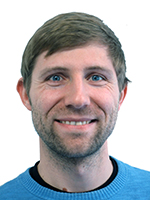
\includegraphics[width=0.25\linewidth]{andreas.jpg}\quad 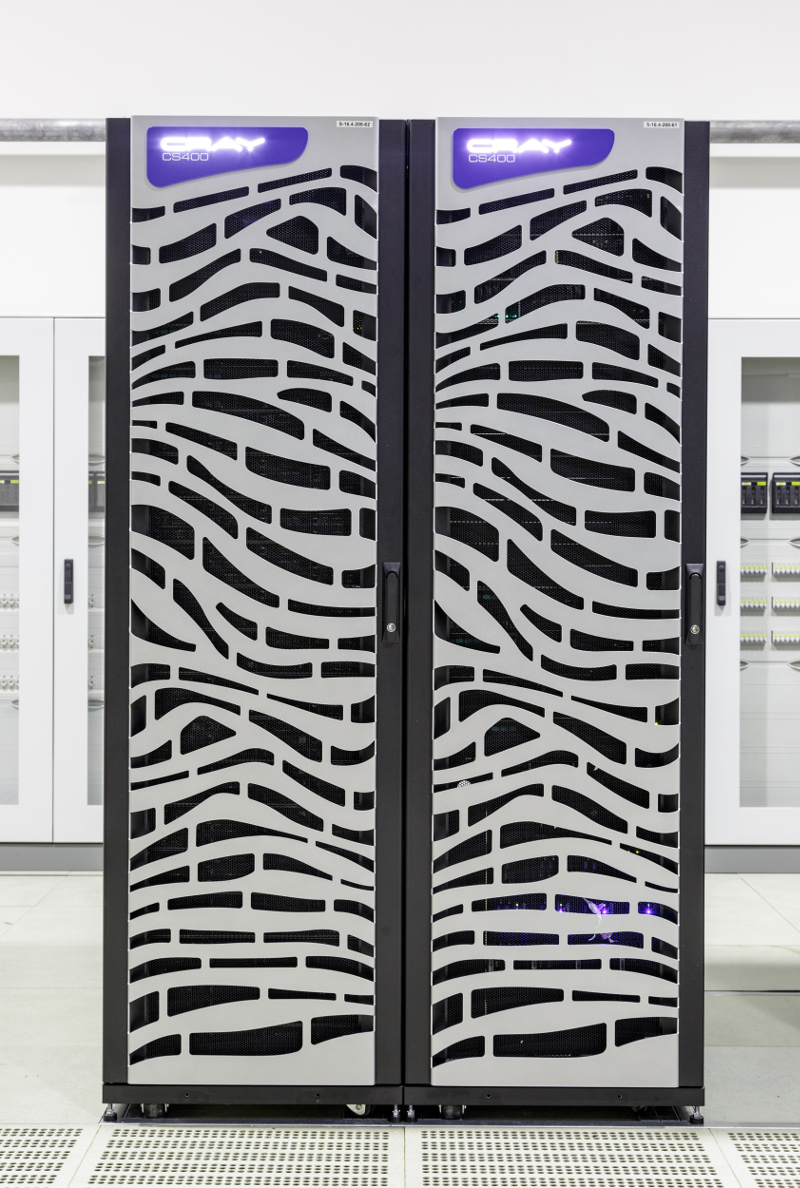
\includegraphics[width=0.25\linewidth]{juron.jpg} \\
        \end{figure}
    \end{column}
\end{columns}
\end{frame}

\end{document}
